\section{Introduzione}
\diapo{La chimica del silicio}
Il silicio come ``{\bf traghettatore}'': 
$$\ce{R ->[?] P}$$
$$\ce{R ->C[+Si] I ->[-\ce{Si}] P}$$
\pause
I {\bf legami del silicio}:
\begin{itemize}
 \item {\bf facile rottura} eterolitica da parte di reagenti ionici, {\bf ossigeno e alogeni};
 \item se {\bf legato al carbonio} può essere considerato un {\bf super-protone};
 \item se {\bf legato all'ossigeno} può essere considerato un {\bf protone indebolito}.
\end{itemize}
\end{frame}


%%%%%%%%%%%%%%%%%%%%%%%%%%%%%%%%%%%%%%%%%%%%%%%%%%%%%%%%%%%%%%%%%%%%
\logo{}

\begin{frame}
\frametitle{La chimica del silicio}
\begin{block}{Effetto $\beta$: ($\sigma$--p)$_\pi$}
\begin{figure}{\centering{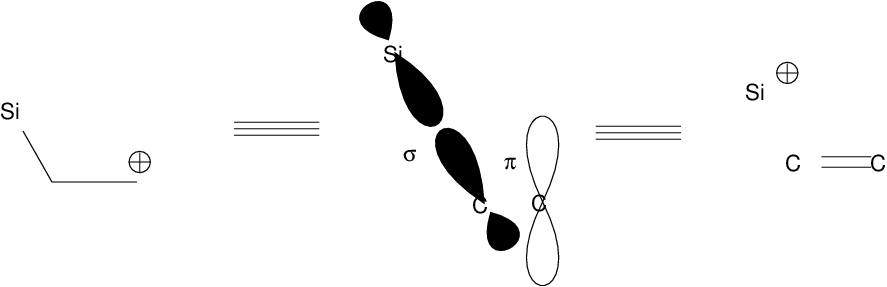
\includegraphics[width=0.7\textwidth]{img/intro/b-effect.png}}}\end{figure}
\end{block}
\pause
\begin{block}{$\alpha$ anioni: ($\sigma$*--p)$_\pi$}
\begin{figure}{\centering{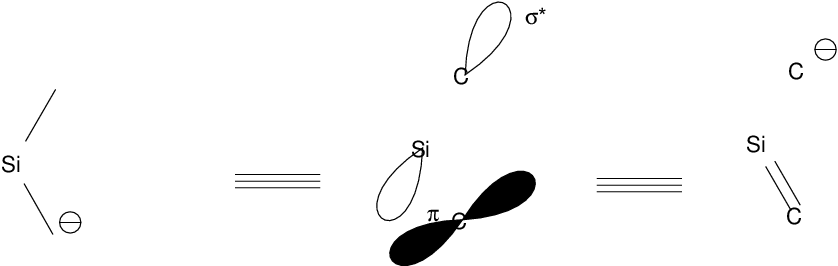
\includegraphics[width=0.7\textwidth]{img/intro/a-anions.png}}}\end{figure}
\end{block}
\end{frame}

\logo{
\includegraphics[width=0.07\paperwidth]{img/snslogo.png}}

%%%%%%%%%%%%%%%%%%%%%%%%%%%%%%%%%%%%%%%%%%%%%%%%%%%%%%%%%%%%%%%%%%%%

\diapo{Schema generale delle reazioni di interesse}
\begin{figure}{\centering{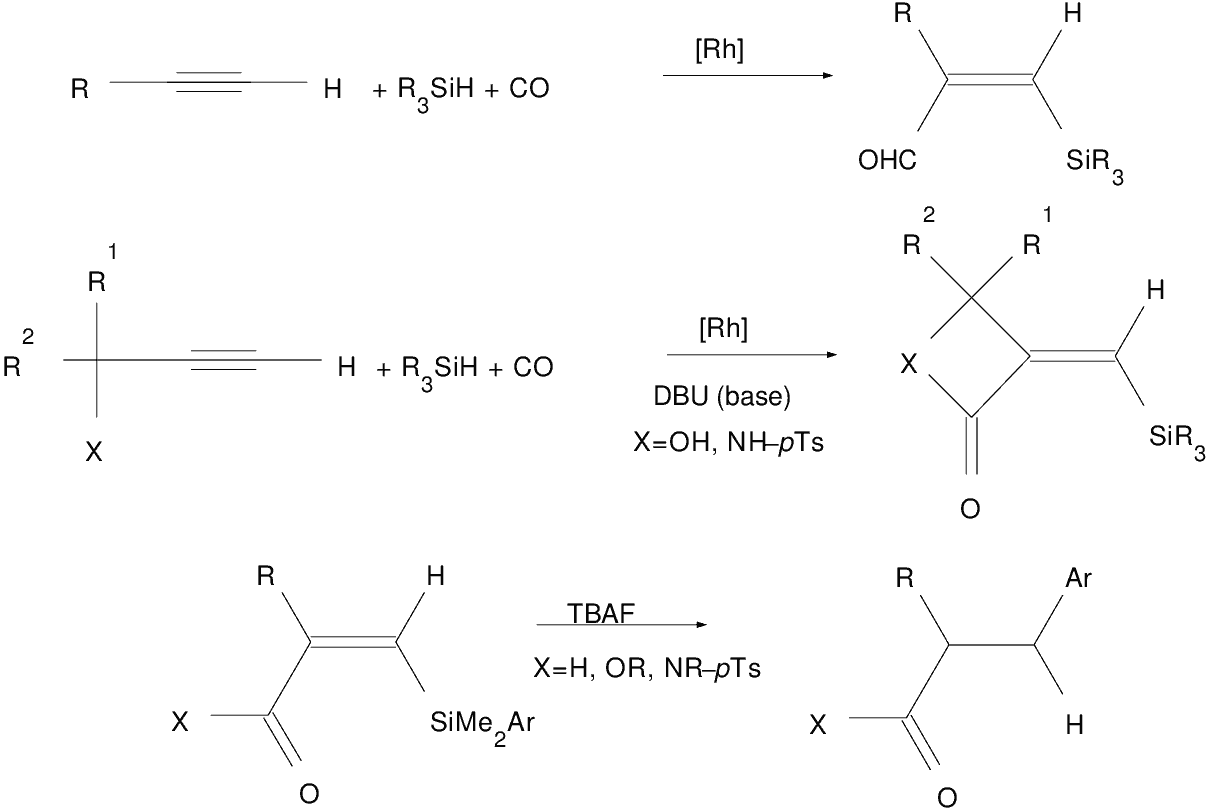
\includegraphics[width=0.8\textwidth]{img/intro/generale.png}}}\end{figure}


\end{frame}

\subsection{Prodotti ottenibili da $\beta$-silil alchenali}\begin{frame}\frametitle{Prodotti ottenibili da $\beta$-silil alchenali}
I $\beta$-sililalchenali ottenuti possono poi essere trasformati sfruttando la {\bf reattività sia di un carbonile $\alpha , \beta $ insaturo sia di un vinil silano}.
\begin{figure}{\centering{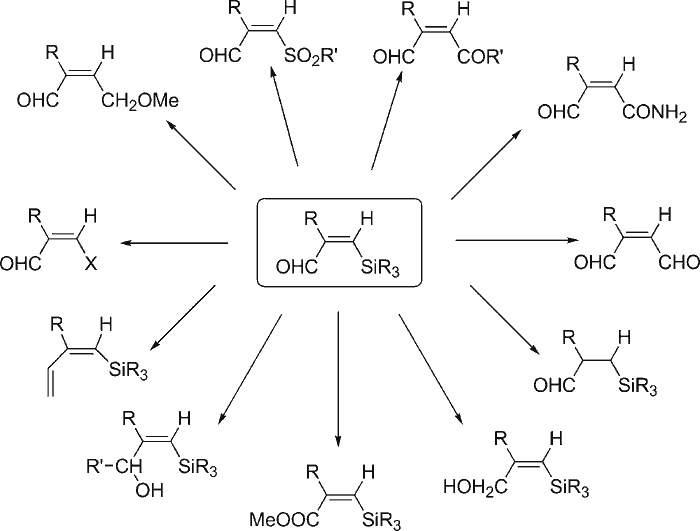
\includegraphics[width=0.6\textwidth]{img/intro/altri_prodotti_ottenibili.png}}}\end{figure}


\end{frame}


%%%%%%%%%%%%%%%%%%%%%%%%%%%%%%%%%%%%%%%%%%%%%%%%%%%%%%%%%%%%%%%%%%%%


